% Editable reconstruction; interpretation recorded in root.json.
% Shared standalone design for the editable figure reconstructions.
\documentclass[tikz,border=5pt,10pt]{standalone}
\usepackage[T1]{fontenc}
\usepackage[utf8]{inputenc}
\usepackage{newpxtext,newpxmath}
\usepackage[scaled=.94]{sourcesanspro}
\usepackage{pgfplots}
\pgfplotsset{compat=1.18}
\usetikzlibrary{arrows.meta,calc,positioning,decorations.pathreplacing,
  decorations.markings,patterns,matrix,shapes.geometric,fit,backgrounds,
  intersections,angles,quotes}
\definecolor{ink}{HTML}{203746}
\definecolor{accent}{HTML}{146C78}
\definecolor{muted}{HTML}{667780}
\definecolor{signalred}{HTML}{B94B44}
\color{ink}
\tikzset{>=Latex,line width=.8pt,
  every node/.style={font=\small},
  axis/.style={->,draw=muted,line width=.5pt},
  guide/.style={draw=muted,dashed,line width=.45pt},
  curve/.style={draw=accent,line width=1pt},
  marker/.style={circle,fill=accent,inner sep=1.5pt},
  labelbox/.style={fill=white,inner sep=2pt}}

\begin{document}

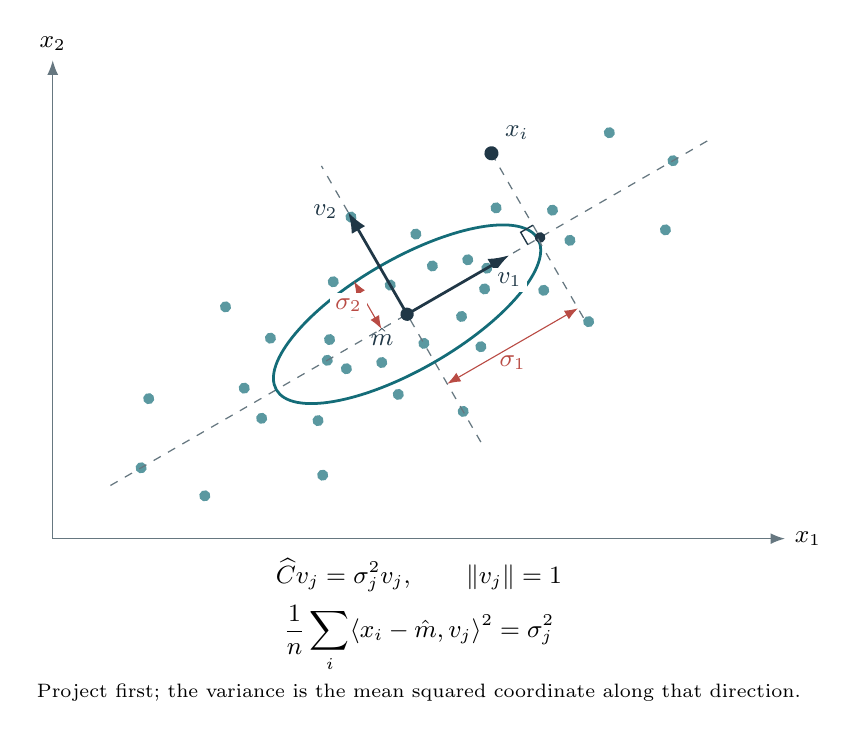
\begin{tikzpicture}[scale=1.5]
% Twelve equally spaced directions at each radius give mean(cos^2)=1/2.
% Standard deviations: (2.6,.95)*sqrt((.3^2+.6^2+1)/6).
\def\sdone{1.2781497043}
\def\sdtwo{.4670162381}
\draw[axis] (-3,-1.9)--(3.2,-1.9) node[right] {$x_1$};
\draw[axis] (-3,-1.9)--(-3,2.15) node[above] {$x_2$};
\begin{scope}[rotate=30]
\foreach \r/\phase in {.3/0,.6/15,1/0}{\foreach \t in {0,30,...,330}{\fill[accent!70] ({2.6*\r*cos(\t+\phase)},{.95*\r*sin(\t+\phase)}) circle(1.35pt);}}
\draw[guide] (-2.9,0)--(3,0) (0,-1.25)--(0,1.45);
\draw[curve] (0,0) ellipse [x radius=\sdone,y radius=\sdtwo];
\coordinate (sample) at (1.3,{.95*sin(60)});
\draw[guide] (sample)--(1.3,0);
\draw[ink,line width=.5pt] (1.18,0)--(1.18,.12)--(1.3,.12);
\fill[ink] (sample) circle(1.7pt) node[above right=2pt] {$x_i$};
\fill[ink] (1.3,0) circle(1.3pt);
\draw[->,ink,line width=1pt] (0,0)--(1,0) node[below=4pt,labelbox] {$v_1$};
\draw[->,ink,line width=1pt] (0,0)--(0,1) node[left] {$v_2$};
\draw[<->,signalred] (0,-.68)--(\sdone,-.68) node[midway,below] {$\sigma_1$};
\draw[guide] (\sdone,0)--(\sdone,-.8);
\draw[<->,signalred] (-.25,0)--(-.25,\sdtwo) node[midway,left,labelbox] {$\sigma_2$};
\fill[ink] (0,0) circle(1.6pt) node[below left=2pt] {$\hat m$};
\end{scope}
\node[align=center] at (.1,-2.55) {$\widehat C v_j=\sigma_j^2v_j,\qquad\|v_j\|=1$\\[4pt]$\displaystyle\frac1n\sum_i\langle x_i-\hat m,v_j\rangle^2=\sigma_j^2$};
\node[font=\scriptsize] at (.1,-3.2) {Project first; the variance is the mean squared coordinate along that direction.};
\end{tikzpicture}
\end{document}
